%
% 言語処理系実験 最終報告用 LaTeX のひな型ファイル
%
% 表紙だけを作るのにも報告書全体を作るのにも使える
%
\documentclass[indiv]{jikken}   % 実験報告用クラスファイル (jikken.cls) が必要
\usepackage[dvipdfmx]{graphicx}  %pngファイルを貼り付けるのに必要
\usepackage[dvipdfmx]{color}
\usepackage{listings, jlisting}
\usepackage{color}
\usepackage{float}
\usepackage{ascmac}
\usepackage{amsmath}

\lstset{
	%プログラム言語(複数の言語に対応,C,C++も可)
 	language = Python,
 	%背景色と透過度
 	backgroundcolor={\color[gray]{.90}},
 	%枠外に行った時の自動改行
 	breaklines = true,
 	%自動改行後のインデント量(デフォルトでは20[pt])	
 	breakindent = 10pt,
 	%標準の書体
 	basicstyle = \ttfamily\scriptsize,
 	%コメントの書体
 	commentstyle = {\itshape \color[cmyk]{1,0.4,1,0}},
 	%関数名等の色の設定
 	classoffset = 0,
 	%キーワード(int, ifなど)の書体
 	keywordstyle = {\bfseries \color[cmyk]{0,1,0,0}},
 	%表示する文字の書体
 	stringstyle = {\ttfamily \color[rgb]{0,0,1}},
 	%枠 "t"は上に線を記載, "T"は上に二重線を記載
	%他オプション:leftline,topline,bottomline,lines,single,shadowbox
 	frame = TBrl,
 	%frameまでの間隔(行番号とプログラムの間)
 	framesep = 5pt,
 	%行番号の位置
 	numbers = left,
	%行番号の間隔
 	stepnumber = 1,
	%行番号の書体
 	numberstyle = \tiny,
	%タブの大きさ
 	tabsize = 4,
 	%キャプションの場所("tb"ならば上下両方に記載)
 	captionpos = t,
    %空白を表示するかどうか
    showstringspaces = false,
}
\setcounter{secnumdepth}{3}  %目次のために必要

%%% 通常は書き換え不要
\renewcommand{\実験名}{パターン認識と機械学習}
\renewcommand{\作成日}{2023年1月31日}
\renewcommand{\学年}{2}
%\renewcommand{\学年}{3}

\newcommand{\本年}{2022年}
\newcommand{\次年}{2023年}

%%%11/29, 12/06, 12/13, 12/20, 01/17, 01/24, 01/31
%%% \num 月 \num 日 を実施日に書き換える
\newcommand{\実施日1}{\本年 11 月 29 日}
\newcommand{\実施日2}{\本年 12 月 6 日}
\newcommand{\実施日3}{\本年 12 月 13 日}
\newcommand{\実施日4}{\本年 12 月 20 日}
\newcommand{\実施日5}{\次年 1 月 17 日}
\newcommand{\実施日6}{\次年 1 月 24 日}
\newcommand{\実施日7}{\次年 1 月 31 日}

%%% {\samplenum}{\samplename} を報告者の番号と氏名に書き換える
\newcommand{\報告者}{\番号と氏名{421858}{若山陽向}}
%%% 言語処理系実験では以下の共同実験者の記述は不要
%\newcommand{\実験者1}{\番号と氏名{\samplenum}{\samplename}}
%\newcommand{\実験者2}{\番号と氏名{\samplenum}{\samplename}}
%\newcommand{\実験者3}{\番号と氏名{\samplenum}{\samplename}}
%\newcommand{\実験者4}{\番号と氏名{\samplenum}{\samplename}}
%\newcommand{\実験者5}{\番号と氏名{\samplenum}{\samplename}}
%\newcommand{\実験者6}{\番号と氏名{\samplenum}{\samplename}}
%\newcommand{\実験者7}{\番号と氏名{\samplenum}{\samplename}}

%%%%%%%%%%%%%%%%%%%%%%%%%%%%%%%%%%%%%%%%%%%%%%%%%%%%%%%%%%%%%%%%%%%%%%%%%%%%%%

\begin{document}

\表紙  % 報告書の表紙を作る

%%% 報告書全体を作るなら以下を書き換える (構成は自由に変えてよい)
%

\tableofcontents  %目次を作る
\clearpage

\begin{section}{目的}     
    今回の目的は、Pythonを使いパターン認識と機械学習の基礎がどのように行われているのか知り
    人工知能関連の研究に対するイメージを付けることと、個別課題を通して問題解決する力を身に付ける事である。
    そのために、Jetson Nanoを使用してプログラム作成を行う。
\end{section}

\begin{section}{このレポートの構成}
    プログラムの結果や解説は第\ref{メイン}章に載せてある。その際、まずはコードを全て載せ、その後に随時解説をしている。\\
    このようにコードを説明するときは一度に載せるのではなく、分割して載せ、その度に説明することで、可読性を向上させた。
\end{section}

\begin{section}{実験方法}
    Jetson NanoにlinuxディストリビューションのDebian系であるUbuntuをインストールして行った。GUIなので使いやすかった。
    コーディングには主にVSCodeを使った。
    理由としては、コーディングが圧倒的にVSCodeがやりやすく、また、Jupyterを使うことも考えたが、全体のコードを
    分割して入力していく方式だと、後々コードを提出することを考えた時に煩わしいので、一度に全部を入力できるVSCodeを使用した。\\

    なお、Pythonのプログラムを実行するときは、動作などはmain関数や他の関数を用意して書いたが、プログラムの最後には必ず
    \begin{lstlisting}
if __name__ == '__main__':
    main()
    \end{lstlisting}
    を付けた。\\
    これをつけることで、python ファイル名.py ではなく、単にそのプログラムがimportされただけの時に処理が実行されることを防ぐことができる。
\end{section}


\begin{section}{実験結果、動作試験、およびプログラムの詳細解説}
    \label{メイン}
    \begin{subsection}{畳み込みフィルタ}

        \begin{lstlisting}
# coding: UTF-8
import cv2
import numpy as np
import time

def main():

    #ここを変えることで他の画像も使える
    before_picture = 'ducks.jpg'

    #SobelYを定義
    SobelY = np.array([[-1, -2, -1], [0, 0, 0], [1, 2, 1]])

    #SobelXを定義
    SobelX = np.array([[-1, 0, 1], [-2, 0, 2], [-1, 0, 1]])

    #Gaussian3を定義
    Gaussian3 = np.array([[1/16, 2/16, 1/16], [2/16, 4/16, 2/16], [1/16, 2/16, 1/16]])

    #Gaussian5を定義
    Gaussian5 = np.array([[1/256, 4/256, 6/256, 4/256, 1/256], [4/256, 16/256, 24/256, 16/256, 4/256], [6/256, 24/256, 36/256, 24/256, 6/256], 
                                            [4/256, 16/256, 24/256, 16/256, 4/256], [1/256, 4/256, 6/256, 4/256, 1/256]])

    img = cv2.imread(before_picture, cv2.IMREAD_GRAYSCALE)  #モノクロで読み取る

    print('処理中です')
    time_begin = time.perf_counter()

    cv2.imwrite('convoluted.jpg', convolution(img, SobelY))

    time_end = time.perf_counter()
    print('終了しました\nconvoluted.jpgに結果を保存しました')
    calc_sec = time_end - time_begin
    print('かかった時間 : ', calc_sec, '秒')


def convolution(img, kernel):
    img_xsize = img.shape[0]
    img_ysize = img.shape[1]
    #グレイスケールなのでz成分はない

    kernel_xsize = kernel.shape[0]
    kernel_ysize = kernel.shape[1]
    
    #最終的にreturnする画像はappended_img
    appended_img = np.zeros((img_xsize + 4, img_ysize + 4)) 
        
    #imgからkernelのサイズ分抜き出した画像の要素の行列
    picked_img = np.array([[0, 0, 0], [0, 0, 0], [0, 0, 0]])

    temp = np.zeros((kernel_xsize, kernel_ysize))

    for i in range(img_xsize):
        for j in range(img_ysize):
            appended_img[i+2, j+2] = img[i, j]
            #appended_imgの内部はimgと同じだが、周囲が0でパディングされているところだけ違う


    for i in range(img_xsize):
        for j in range(img_ysize):
            picked_img = appended_img[i: i+kernel_xsize, j: j+kernel_ysize]  #imgからkernelサイズ分抜き出す
            temp = np.multiply(picked_img, kernel)  #picked_imgとkernelのアダマール積を求める
            appended_img[i, j] = np.sum(temp)  #先程のtempの全成分の和を代入する

    return appended_img

if __name__ == '__main__':
    main()         
        \end{lstlisting}

        まずは、次のようにカーネルを定義した。
        \begin{lstlisting}
#SobelYを定義
SobelY = np.array([[-1, -2, -1], [0, 0, 0], [1, 2, 1]])

#SobelXを定義
SobelX = np.array([[-1, 0, 1], [-2, 0, 2], [-1, 0, 1]])

#Gaussian3を定義
Gaussian3 = np.array([[1/16, 2/16, 1/16], [2/16, 4/16, 2/16], [1/16, 2/16, 1/16]])

#Gaussian5を定義
Gaussian5 = np.array([[1/256, 4/256, 6/256, 4/256, 1/256], [4/256, 16/256, 24/256, 16/256, 4/256], [6/256, 24/256, 36/256, 24/256, 6/256], 
                                        [4/256, 16/256, 24/256, 16/256, 4/256], [1/256, 4/256, 6/256, 4/256, 1/256]])
        \end{lstlisting}

        
        次に、画像をモノクロで読み取り、
        \begin{lstlisting}
img = cv2.imread(before_picture, cv2.IMREAD_GRAYSCALE)
        \end{lstlisting}


        関数\verb|convolution()|を呼び出し計算させた。また、関数\verb|time.perf_counter()|を用いて計算時間を算出した。
        フィルターをかけた後の画像は\verb|convoluted.jpg|に保存した。
        
        \begin{lstlisting}
print('処理中です')
time_begin = time.perf_counter()

cv2.imwrite('convoluted.jpg', convolution(img, SobelY))

time_end = time.perf_counter()
print('終了しました\nconvoluted.jpgに結果を保存しました')
calc_sec = time_end - time_begin
print('かかった時間 : ', calc_sec, '秒')
        \end{lstlisting}

        
        ここから、関数\verb|convolution()|の説明をする。まずはカーネルのサイズを\verb|shape|で取得する。
        x方向の大きさは\verb|kernel.shape[0]|に、y方向の大きさは\verb|kernel.shape[1]|にあるので、それぞれ取得した。
        \begin{lstlisting}
kernel_xsize = kernel.shape[0]
kernel_ysize = kernel.shape[1]
        \end{lstlisting}

        
        最終的に\verb|return|する画像、つまりフィルタをかけた後の画像は\verb|appended_img|であるが、そのサイズは、x方向y方向ともに4ずつ伸ばした。
        今回使うカーネルの最大は\verb|Gaussian5|の5 $\times$ 5であり、畳み込み演算を行う時に使うサイズは3 $\times$ 3、よって2足りない。
        この足りない2がx方向だと左右、y方向だと上下にあるので、足りない2に$\times$2をして4となるから、それらを追加したサイズとした。
        
        \begin{lstlisting}
appended_img = np.zeros((img_xsize + 4, img_ysize + 4))  
        \end{lstlisting}


        次の処理は、元々の\verb|img|のままだと、フィルタをかける時に端までかけることができないので、元々の画像の周囲を0でパディングしている。
        \begin{lstlisting}
for i in range(img_xsize):
    for j in range(img_ysize):
        appended_img[i+2, j+2] = img[i, j]
        #appended_imgの内部はimgと同じだが、周囲が0でパディングされているところだけ違う。
        \end{lstlisting}


        ここからは計算部分である。
        \begin{lstlisting}
for i in range(img_xsize):
    for j in range(img_ysize):

        #imgからkernelサイズ分抜き出す
        picked_img = appended_img[i: i+kernel_xsize, j: j+kernel_ysize]

        #picked_imgとkernelのアダマール積を求める
        temp = np.multiply(picked_img, kernel)  

        #先程のtempの全成分の和を代入する
        appended_img[i, j] = np.sum(temp)  

    return appended_img
        \end{lstlisting}
        ここで、アダマール積の説明をする。アダマール積とは、行列の同じ部分の要素のみ掛け合わせる演算である。\\


        例えば、
        \begin{math}
            \begin{bmatrix}
                1 & 2 & 3 \\
                4 & 5 & 6 \\
                7 & 8 & 9 \\
            \end{bmatrix}
            \bigodot
            \begin{bmatrix}
                10 & 11 & 12 \\
                13 & 14 & 15 \\
                16 & 17 & 18 \\
            \end{bmatrix}
        \end{math}
        のような計算を考えてみる。($\bigodot$はアダマール積の演算を示す。)\\


        答えの(1,1)成分は1$\times$10なので10、(1,2)成分は2$\times$11なので22という様に考えるので、答えは
        \begin{math}
            \begin{bmatrix}
                1 \times 10 = 10 & 2 \times 11 = 22 & 3 \times 12 = 36 \\
                4 \times 13 = 52 & 5 \times 14 = 70 & 6 \times 15 = 90 \\
                7 \times 16 = 112 & 8 \times 17 = 136 & 9 \times 18 = 162 \\
            \end{bmatrix}
        \end{math}
        となる。\\

        以上を踏まえると、この部分ではまず先程パディングした\verb|appended_img|をカーネルのサイズで切り出し、それとカーネル
        とのアダマール積を求めている。あとはアダマール積の演算でできた配列\verb|temp|の全要素の和を算出すれば、求めたい要素の
        値になる。
        分かりやすくするために、参考にしたサイトに書き込んだ画像を貼り付ける。(出典 : \cite[畳み込み演算]{畳み込み演算})
        \begin{figure}[H]
            \begin{center}
             \resizebox{12cm}{!}{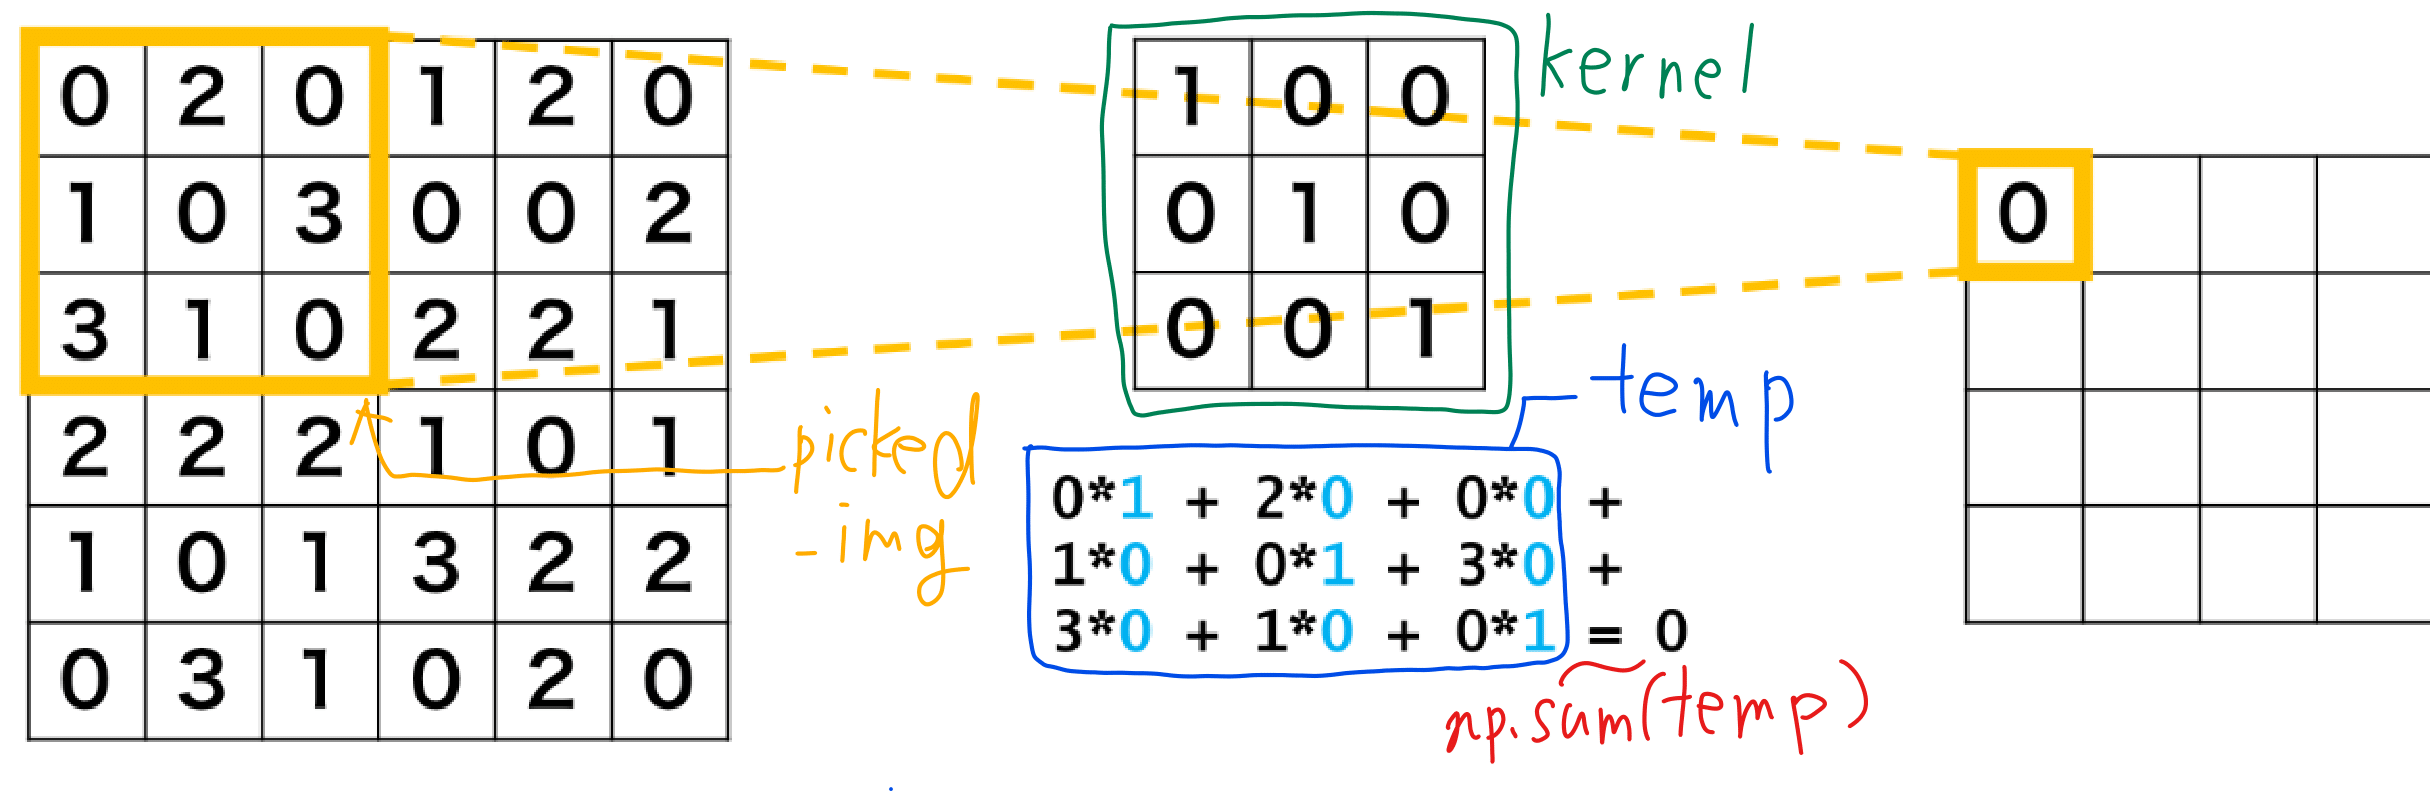
\includegraphics{kernel_calc.png}}
             \caption{参考図}\label{picture:kernel_calc}
            \end{center}
        \end{figure}

        ここから、各カーネルの結果を示す。まずは、元々の画像を貼る。
        \begin{figure}[H]
            \begin{center}
             \resizebox{12cm}{!}{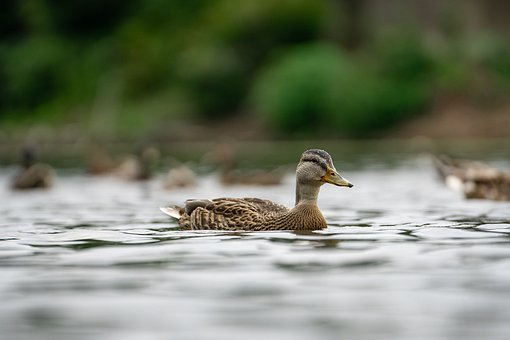
\includegraphics{ducks.jpg}}
             \caption{フィルタ前の画像}\label{picture:ducks}
            \end{center}
        \end{figure}

        ここからはフィルタをかけている画像である。\\
        1. SobelY
        \begin{figure}[H]
            \begin{center}
             \resizebox{8cm}{!}{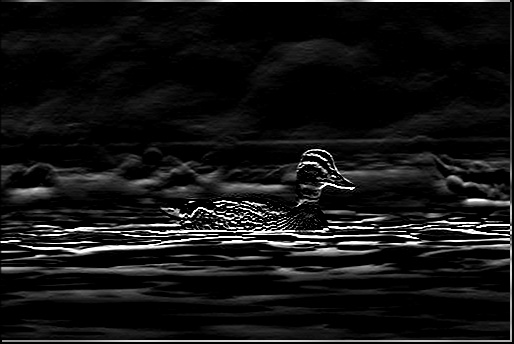
\includegraphics{convoluted_SobelY.jpg}}
             \caption{SobelYの画像}\label{picture:convoluted_SobelY}
            \end{center}
        \end{figure}

        2. SobelX
        \begin{figure}[H]
            \begin{center}
             \resizebox{8cm}{!}{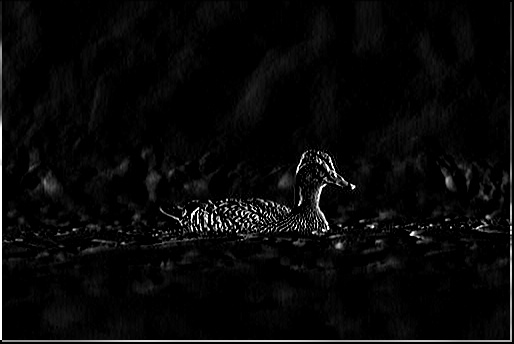
\includegraphics{convoluted_SobelX.jpg}}
             \caption{SobelXの画像}\label{picture:convoluted_SobelX}
            \end{center}
        \end{figure}

        3. Gaussian3
        \begin{figure}[H]
            \begin{center}
             \resizebox{8cm}{!}{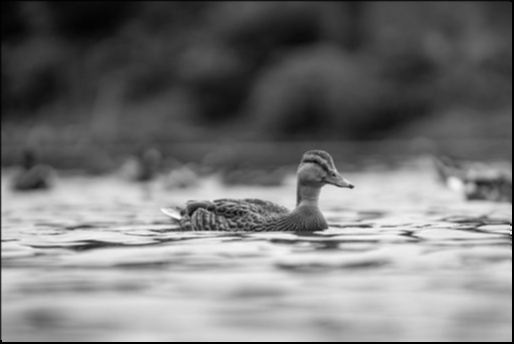
\includegraphics{convoluted_Gaussian3.jpg}}
             \caption{Gaussian3の画像}\label{picture:convoluted_Gaussian3}
            \end{center}
        \end{figure}

        4. Gaussian5
        \begin{figure}[H]
            \begin{center}
             \resizebox{8cm}{!}{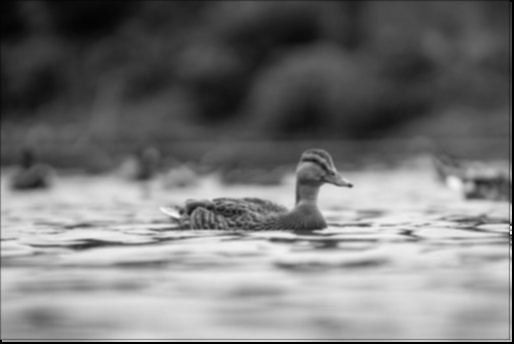
\includegraphics{convoluted_Gaussian5.jpg}}
             \caption{Gaussian5の画像}\label{picture:convoluted_Gaussian5}
            \end{center}
        \end{figure}
        確かに、スライドと同じようなフィルタを通した後の結果が得られたことが分かる。


    \end{subsection}
    \begin{subsection}{最急降下法}
        \begin{subsubsection}{基礎}
        \label{基礎課題2}
        \begin{lstlisting}
#!/usr/bin/python3
# coding: UTF-8
import cv2
import math
import time

def main():
    check_f1()
    check_f2()

def check_f1():
    eta = pow(10, -3)  #収束速度定数は10^-3にした
    exist_minimum = True  #最小値が存在するか(存在しないのならFalse)

    f1_minimum_list = []  #f1の最小値を格納するリスト
    minimum_x_list = []  #xの最小値を格納するリスト
        #複数の初期値からなので、-10~10までで試す
    for begin_init in range(-10, 10):
        x = begin_init
        for i in range(10000):
            x -= eta * d_f1(x)
            if( f1(x) > pow(2, 31)):  #2^31を超えると流石にでかすぎて答えとして不適なのでbreakする
                break
            if( f1(x) < -pow(2,31)):  #-(2^31)より小さいと最小値なしと判定
                exist_minimum = False
                break
        f1_minimum_list.append(f1(x))  #結果をlistに付け加えておく
        minimum_x_list.append(x)  #結果をlistに付け加えておく

    if( exist_minimum == True ):
        print('2x^2+8x-16の最小値は ', min(f1_minimum_list))  #listの最小値を出す
        min_index = f1_minimum_list.index(min(f1_minimum_list))  #minの時の添字を出す
        print('その際のx = ', minimum_x_list[min_index], '\n')
    else:
        print('2x^2+8x-16の最小値は存在しません\n')

    

def check_f2():
    eta = pow(10, -3)  #収束速度定数は10^-3にした
    exist_minimum = True  #最小値が存在するか(存在しないのならFalse)

    f2_minimum_list = []  #f1の最小値を格納するリスト
    minimum_x_list = []  #xの最小値を格納するリスト
    exist_minimum = True 
    #複数の初期値からなので、-10~10までで試す
    for begin_init in range(-10, 10):
        x = begin_init
        for i in range(10000):
            x -= eta * d_f2(x)
            if( f2(x) > pow(2, 31)):  #2^31を超えると流石にでかすぎて答えとして不適なのでbreakする
                break
            if( f2(x) < -pow(2,31)):  #-(2^31)より小さいと最小値なしと判定
                exist_minimum = False
                break
        f2_minimum_list.append(f2(x))  #結果をlistに付け加えておく
        minimum_x_list.append(x)  #結果をlistに付け加えておく

    if( exist_minimum == True ):
        print('2x^2+8x-16の最小値は ', min(f2_minimum_list))  #listの最小値を出す
        min_index = f2_minimum_list.index(min(f2_minimum_list))  #minの時の添字を出す
        print('その際のx = ', minimum_x_list[min_index], '\n')
    else:
        print('2x^2+8x-16の最小値は存在しません')



def f1(x):
    return 2*pow(x, 2) + 8*x - 16

def d_f1(x):
    return 4*x + 8

def f2(x):
    return pow(x, 3)- 4*pow(x, 2) + x - 2

def d_f2(x):
    return 3*pow(x, 2) - 8*x + 1

if __name__ == '__main__':
    main()         
        \end{lstlisting}

        次に、再急降下法について考える。まず、収束速度定数は$10^{-3}$にした。
        \begin{lstlisting}
#収束速度定数は10^-3にした
eta = pow(10, -3)
        \end{lstlisting}

        続いて\verb|bool|型の変数\verb|exist_minimum|を定義し、最小値が存在するかを判定させた。
        どのように判定するかは後述する。
        \begin{lstlisting}
#最小値が存在するか(存在するならTrue)
exist_minimum = True
        \end{lstlisting}

        初期値に対する依存性を調べるため、複数の初期値から開始しているのが次の部分である。
        \begin{lstlisting}
#複数の初期値からなので、-10~10までで試す
for begin_init in range(-10, 10):
    x = begin_init
        \end{lstlisting}    
                
        再急降下法は1次収束であり、局所的最適解にたどり着くまでに必要な反復回数が多くなりやすいことが知られている。
        (出典 : \cite[再急降下法]{再急降下法})\\
        そのため、ニュートン法と比較すると収束までが遅い。
        よって、反復回数は10000回と多めに設定した。
        \begin{lstlisting}
for begin_init in range(-10, 10):
    x = begin_init
    for i in range(10000):
        \end{lstlisting}

        続いて、定義式
        \begin{equation}
            x \leftarrow x - \eta \frac{df(x)}{dx}
        \end{equation}
        とあるように、4行目の\verb|x -= eta * d_f1(x)|でその計算を行っている。\\
        5行目以降は極端な値になった時の処理である。
        特に、下のif文は、$-(2^{31})$より小さいと最小値なしと判定し、最小値の有無を示す変数\verb|exist_minimum|を\verb|False|にしている。
        これにより、最小値が存在しない事を記録することができる。
        \begin{lstlisting}
for begin_init in range(-10, 10):
    x = begin_init
    for i in range(10000):
    x -= eta * d_f1(x)
        if( f1(x) > pow(2, 31)):  #2^31を超えると流石にでかすぎて答えとして不適なのでbreakする
            break
        if( f1(x) < -pow(2,31)):  #-(2^31)より小さいと最小値なしと判定
            exist_minimum = False
            break
        \end{lstlisting}

        また、その時のf1(x), xの値は\verb|append|を使用して記録しておく。
        \begin{lstlisting}
for begin_init in range(-10, 10):
    x = begin_init
    for i in range(10000):
        x -= eta * d_f1(x)
        if( f1(x) > pow(2, 31)):  #2^31を超えると流石にでかすぎて答えとして不適なのでbreakする
            break
        if( f1(x) < -pow(2,31)):  #-(2^31)より小さいと最小値なしと判定
            exist_minimum = False
            break
    f1_minimum_list.append(f1(x))  #結果をlistに付け加えておく
    minimum_x_list.append(x)  #結果をlistに付け加えておく
        \end{lstlisting}

        最後に、変数\verb|exist_minimum|の値によって最小値を表示するかどうかを判定している。
        その際、\verb|index|を用いて添え字を取得した。
        \begin{lstlisting}        
if( exist_minimum == True ):
    print('2x^2+8x-16の最小値は ', min(f1_minimum_list))  #listの最小値を出す
    min_index = f1_minimum_list.index(min(f1_minimum_list))  #minの時の添字を出す
    print('その際のx = ', minimum_x_list[min_index], '\n')
else:
    print('2x^2+8x-16の最小値は存在しません\n')
        \end{lstlisting}

        \verb|f2|については、\verb|f1|と考え方は全く同じなので詳細な解説は省略する。変更点は、\verb|f1|を\verb|f2|にしたところと、\verb|f1|における
        \begin{lstlisting}
if( exist_minimum == True ):
    print('2x^2+8x-16の最小値は ', min(f1_minimum_list))  #listの最小値を出す
    min_index = f1_minimum_list.index(min(f1_minimum_list))  #minの時の添字を出す
    print('その際のx = ', minimum_x_list[min_index], '\n')
else:
    print('2x^2+8x-16の最小値は存在しません\n')
        \end{lstlisting}
        を
        \begin{lstlisting}
if( exist_minimum == True ):
    print('x^3-4x^2+x-2の最小値は ', min(f2_minimum_list))  #listの最小値を出す
    min_index = f2_minimum_list.index(min(f2_minimum_list))  #minの時の添字を出す
    print('その際のx = ', minimum_x_list[min_index], '\n')
else:
    print('x^3-4x^2+x-2の最小値は存在しません')
        \end{lstlisting}
        に変更したところである。

        また、\verb|f1(), d_f1(), f2(), d_f2()|は次のように定義している。
        \begin{lstlisting}
def f1(x):
    return 2*pow(x, 2) + 8*x - 16

def d_f1(x):
    return 4*x + 8

def f2(x):
    return pow(x, 3)- 4*pow(x, 2) + x - 2

def d_f2(x):
    return 3*pow(x, 2) - 8*x + 1
        \end{lstlisting}
        要するに、\verb|d_f1(x)|には\verb|f1(x)|を\verb|x|について微分した値が入っていて、
        \verb|d_f2(x)|には\verb|f2(x)|を\verb|x|について微分した値が入っている。\\

        
        このプログラムの実行結果を以下に示す。
        
        \begin{verbatim}
2x^2+8x-16の最小値は  -24.0
その際のx =  -2.000000000000055

2x^2+8x-16の最小値は存在しません
        \end{verbatim}

        \end{subsubsection}

        \begin{subsubsection}{発展}
        \begin{lstlisting}
#!/usr/bin/python3
# coding: UTF-8
import cv2
import math
import time


def main():
    eta = pow(10, -3)  #収束速度定数は10^-3にした
    exist_minimum = True  #最小値が存在するか(存在しないのならFalse)

    minimum_list = []  #最小値を格納するリスト
    minimum_x_list = []  #xの最小値を格納するリスト
    minimum_y_list = []  #yの最小値を格納するリスト

    #複数の初期値からなので、-10~10までで試す
    for begin_init in range(-10, 10):
        x = begin_init
        y = begin_init
        for i in range(10000):
            x -= eta * d_f(x, y)
            y -= eta * d_f(x, y)
            if( x > pow(2, 31) or y > pow(2, 31)):  #2^31を超えると流石に大きすぎて答えとして不適なのでbreakする
                break
            if( f(x, y) < -pow(2,31)):  #-(2^31)より小さいと最小値なしと判定
                exist_minimum = False
                break
        minimum_list.append(f(x, y))  #結果をlistに付け加えておく
        minimum_x_list.append(x)  #結果をlistに付け加えておく
        minimum_y_list.append(y)  #結果をlistに付け加えておく

    if( exist_minimum == True ):
        print('(1-x)^2 + 100(y-x^2)^2の最小値は', min(minimum_list))  #listの最小値を出す
        min_index = minimum_list.index(min(minimum_list))  #minの時の添字を出す
        print('その際のx = ', minimum_x_list[min_index])
        print('その際のy = ', minimum_y_list[min_index])
    else:
        print('(1-x)^2 + 100(y-x^2)^2の最小値は存在しません\n')
    

def f(x, y):
    return pow((1-x), 2) + 100*pow(y - pow(x, 2), 2)  #つまり、(1-x)^2 + 100(y - x^2)^2

def d_f(x, y):
    return 400*pow(x, 3) - 200*pow(x, 2) + 2*x - 400*x*y - 2 + 200*y

if __name__ == '__main__':
    main()         
        \end{lstlisting}

        基本的な考え方は\ref{基礎課題2}と同じだが、2変数になったので、若干コード量が増えている。例えば、基礎課題2のf1の方は
        \begin{lstlisting}
for begin_init in range(-10, 10):
    x = begin_init
    for i in range(10000):
        x -= eta * d_f1(x)
        if( f1(x) > pow(2, 31)):  #2^31を超えると流石にでかすぎて答えとして不適なのでbreakする
            break
        if( f1(x) < -pow(2,31)):  #-(2^31)より小さいと最小値なしと判定
            exist_minimum = False
            break
    f1_minimum_list.append(f1(x))  #結果をlistに付け加えておく
    minimum_x_list.append(x)  #結果をlistに付け加えておく
        \end{lstlisting}
        となっていたが、この部分は

        \begin{lstlisting}
#複数の初期値からなので、-10~10までで試す
for begin_init in range(-10, 10):
    x = begin_init
    y = begin_init
    for i in range(10000):
        x -= eta * d_f(x, y)
        y -= eta * d_f(x, y)
        if( x > pow(2, 31) or y > pow(2, 31)):  #2^31を超えると流石に大きすぎて答えとして不適なのでbreakする
            break
        if( f(x, y) < -pow(2,31)):  #-(2^31)より小さいと最小値なしと判定
            exist_minimum = False
            break
    minimum_list.append(f(x, y))  #結果をlistに付け加えておく
    minimum_x_list.append(x)  #結果をlistに付け加えておく
    minimum_y_list.append(y)  #結果をlistに付け加えておく
        \end{lstlisting}
        とあるように、変数\verb|y|に関するコードを増やした。また、基礎課題2のf1で最小値を出す部分は

        \begin{lstlisting}
if( exist_minimum == True ):
    print('2x^2+8x-16の最小値は ', min(f1_minimum_list))  #listの最小値を出す
    min_index = f1_minimum_list.index(min(f1_minimum_list))  #minの時の添字を出す
    print('その際のx = ', minimum_x_list[min_index], '\n')
else:
    print('2x^2+8x-16の最小値は存在しません\n')
        \end{lstlisting}
        となっていたのに対し、発展課題2は

        \begin{lstlisting}
if( exist_minimum == True ):
    print('(1-x)^2 + 100(y-x^2)^2の最小値は', min(minimum_list))  #listの最小値を出す
    min_index = minimum_list.index(min(minimum_list))  #minの時の添字を出す
    print('その際のx = ', minimum_x_list[min_index])
    print('その際のy = ', minimum_y_list[min_index])
else:
    print('(1-x)^2 + 100(y-x^2)^2の最小値は存在しません\n')
        \end{lstlisting}
        と、これも変数\verb|y|に関するコードを増やしている。\\

        次に、関数\verb|f(), d_f()|についてだが、まず\verb|f()|については
        \begin{lstlisting}       
def f(x, y):
    return pow((1-x), 2) + 100*pow(y - pow(x, 2), 2)  #つまり、(1-x)^2 + 100(y - x^2)^2
        \end{lstlisting}
        とあるように、問題文の式
        \begin{equation}
            f(x, y) = (a-x)^{2} + b(y-x^{2})^{2} = (1-x)^{2} + 100(y-x^{2})^{2}
        \end{equation}
        にa = 1, b = 100を代入している。\\

        また、\verb|d_f()|については2変数関数の微分公式
        \begin{equation}
            \nabla f(x, y) = \frac{df(x, y)}{dx} + \frac{df(x, y)}{dy}
        \end{equation}
        を用いて計算できるから、

        \begin{equation}
            \begin{split}
            \frac{df(x, y)}{dx} &= -2 + 2x + 100(-4xy + 4x^{3}) \\
            \frac{df(x, y)}{dy} &= 100(2y - 2x^{2})
            \end{split}
        \end{equation}
        を代入して整理すると、

        \begin{equation}
            \begin{split}
            \nabla f(x, y) &= -2 + 2x + 100(-4xy + 4x^{3}) + 100(2y - 2x^{2}) \\
            &= 400x^{3} - 200x^{2} + 2x -400xy -2 +200y 
            \end{split}
        \end{equation}
        となる。したがって、関数\verb|d_f()|は
        \begin{lstlisting}
def d_f(x, y):
    return 400*pow(x, 3) - 200*pow(x, 2) + 2*x - 400*x*y - 2 + 200*y
        \end{lstlisting}
        のように書ける。
            

    このプログラムの実行結果を以下に示す。
        
        \begin{verbatim}
(1-x)^2 + 100(y-x^2)^2の最小値は 0.0
その際のx =  1.0
その際のy =  1.0
        \end{verbatim}
        
        \end{subsubsection}
        
    \end{subsection}

    \begin{subsection}{手書き文字認識}
    \label{手書き文字認識}

    \begin{lstlisting}
#!/usr/bin/python3
# coding: UTF-8
import cv2
import tensorflow.keras
from tensorflow.keras.datasets import cifar10
from tensorflow.keras.models import Sequential
from tensorflow.keras.layers import Dense, Dropout, Flatten
from tensorflow.keras.layers import Conv2D, MaxPooling2D
from tensorflow.keras import backend as K

def main():
    (x_train, y_train), (x_valid, y_valid) = cifar10.load_data()

    x_train = x_train.astype('float32')
    x_train /= 255
    x_valid = x_valid.astype('float32')
    x_valid /= 255

    #x_train = x_train.reshape(x_train.shape[0], x_train.shape[1], x_train.shape[2], 1)
    x_train = x_train.reshape(x_train.shape[0], x_train.shape[1], x_train.shape[2], 3)
    #x_valid = x_valid.reshape(x_valid.shape[0], x_valid.shape[1], x_valid.shape[2], 1)
    x_valid = x_valid.reshape(x_valid.shape[0], x_valid.shape[1], x_valid.shape[2], 3)

    y_1hot_train = tensorflow.keras.utils.to_categorical(y_train, 10)
    y_1hot_valid = tensorflow.keras.utils.to_categorical(y_valid, 10)

    model = Sequential()
    model.add(Conv2D(32, kernel_size = (3,3),
                        activation = 'relu',
                        input_shape = (x_train.shape[1], x_train.shape[2], x_train.shape[3] )))  
    model.add(Conv2D(16, (3,3), activation = 'relu'))
    model.add(MaxPooling2D(pool_size = (2, 2)))
    model.add(Dropout(0.5))
    model.add(Flatten())
    model.add(Dense(256, activation = 'relu'))
    model.add(Dropout(0.2))
    model.add(Dense(64, activation = 'relu'))
    model.add(Dropout(0.3))
    model.add(Dense(32, activation = 'relu'))
    model.add(Dropout(0.3))
    model.add(Dense(10, activation = 'softmax'))

    model.compile(
        loss=tensorflow.keras.losses.categorical_crossentropy,
        optimizer=tensorflow.keras.optimizers.Adam(),
        metrics=['accuracy'])

    model.fit(x_train, y_1hot_train,
                batch_size=128,  
                epochs=32,
                verbose=1,
                validation_data=(x_valid, y_1hot_valid))

    score = model.evaluate(x_valid, y_1hot_valid, verbose=0)
    print('Loss :', score[0])
    print('Accuracy :', score[1])

if __name__ == '__main__':
    main()          
    \end{lstlisting}
    
    まずは次のように
    \begin{lstlisting}
import cv2
import tensorflow.keras
from tensorflow.keras.datasets import mnist
from tensorflow.keras.models import Sequential
from tensorflow.keras.layers import Dense, Dropout, Flatten
from tensorflow.keras.layers import Conv2D, MaxPooling2D
from tensorflow.keras import backend as K
    \end{lstlisting}
    色々と必要な物をimportしておく。
    続いて、関数\verb|mnist.load_data()|を用いて値を読み込んだ後に、\verb|x_train|と\verb|x_valid|を255で除算しておく。
    \begin{lstlisting}
(x_train, y_train), (x_valid, y_valid) = mnist.load_data()

x_train = x_train.astype('float32')
x_train /= 255
x_valid = x_valid.astype('float32')
x_valid /= 255
    \end{lstlisting}

    次に、スライド24枚目の
    \verb|images = images.reshape(img_num, img_rows, img_cols, 1)|の部分は、
    \begin{lstlisting}
x_train = x_train.reshape(x_train.shape[0], x_train.shape[1], x_train.shape[2], 1)
x_valid = x_valid.reshape(x_valid.shape[0], x_valid.shape[1], x_valid.shape[2], 1)
    \end{lstlisting}
    のように、データ数が\verb|shape[0]|、画像の高さが\verb|shape[1]|、画像の幅が\verb|shape[2]|に対応している。
    
    続いて、\verb|y_train|や\verb|y_valid|をone-hot-vector形式に変換する。
    変換した後の変数は分かりやすいように、\verb|1hot_|を変数名に追加した。
    \begin{lstlisting}
y_1hot_train = tensorflow.keras.utils.to_categorical(y_train, 10)
y_1hot_valid = tensorflow.keras.utils.to_categorical(y_valid, 10)
    \end{lstlisting}

    次の部分はMNIST識別用モデルを構築しているところである。
    \begin{lstlisting}
model = Sequential()
    model.add(Conv2D(4, kernel_size = (3,3),
                        activation = 'relu',
                        input_shape = (x_train.shape[1], x_train.shape[2], x_train.shape[3] )))  
    model.add(Conv2D(8, (3, 3), activation = 'relu'))
    model.add(MaxPooling2D(pool_size = (2, 2)))
    model.add(Dropout(0.25))
    model.add(Flatten())
    model.add(Dense(32, activation = 'relu'))
    model.add(Dropout(0.5))
    model.add(Dense(10, activation = 'softmax'))
    \end{lstlisting}
    9行目の\verb|Dense()|の第1引数は16ですると正答率が悪かったので、32に変更した。
    また、11行目の\verb|num_classes|は今回は10である。

    続いて、学習方法を設定した。
    \begin{lstlisting}
model.compile(
    loss=tensorflow.keras.losses.categorical_crossentropy,
    optimizer=tensorflow.keras.optimizers.Adam(),
    metrics=['accuracy'])
    \end{lstlisting}
    SGDとしてスライドではAdadeltaが使用されていたが、正答率が17\%と非常に悪かった。
    後述する\verb|epochs|の数を16に増やしても32\%とそれほど向上しなかった。
    よって、次の資料を参考にして、Adamを選択した。(出典 : \cite[Adamを選択した理由]{Adamを選択した理由})\\
    これにより、正答率が96\%と大幅に向上した。

    そして、学習を実行させた。
    \begin{lstlisting}
model.fit(x_train, y_1hot_train,
    batch_size=128,
    epochs=4,
    verbose=1,
    validation_data=(x_valid, y_1hot_valid))
    \end{lstlisting}
    \verb|y|の方の変数は\verb|x|とは違い、one-hot-vector形式の方を使うことに注意した。\\
    また、\verb|batch_size|は4だと小さすぎる。
    これだと1回に計算するデータの数が少なすぎて、各データに最適化されてしまうので128にした。
    \verb|epochs|の値は、何回学習させるかを示しているが、課題3ではそれほど大きくしなくても十分な正答率が得られたので、
    少なめの値にしている。

    最後に、精度を評価した。
    \begin{lstlisting}
score = model.evaluate(x_valid, y_1hot_valid, verbose=0)
print('Loss :', score[0])
print('Accuracy :', score[1])
    \end{lstlisting}
    評価用データ\verb|images|は\verb|x_valid|に、正解ラベル\verb|labels|は\verb|y_1hot_valid|にそれぞれ入っている。\\
        
    このプログラムを実行した結果を以下に示す。
    \begin{figure}[H]
        \begin{center}
         \resizebox{12cm}{!}{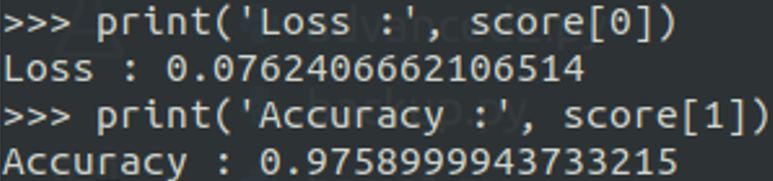
\includegraphics{handwriting_recog_result.png}}
         \caption{手書き文字認識 結果}\label{picture:handwriting_recog_result}
        \end{center}
    \end{figure}

    確かに、\verb|Accuracy|の値が90\%以上になっている事が分かる。\\
    課題の条件である
    \begin{itemize}
        \item 畳み込み層を含むニューラルネットワークを用いている。
        \item Jetson Nano 上でGPUを用いて学習が動作する。
        \item 汎化性能(\verb|Accuracy|の値が90\%以上を達成している。
    \end{itemize}
    は全て満たしている事が分かる。

    \end{subsection}
\end{section}

\begin{section}{自己設定課題}
    \begin{subsection}{導入}
    \label{自己設定課題}
    \begin{lstlisting}
#!/usr/bin/python3
# coding: UTF-8
import cv2
import tensorflow.keras
from tensorflow.keras.datasets import cifar10
from tensorflow.keras.models import Sequential
from tensorflow.keras.layers import Dense, Dropout, Flatten
from tensorflow.keras.layers import Conv2D, MaxPooling2D
from tensorflow.keras import backend as K
    
def main():
    (x_train, y_train), (x_valid, y_valid) = mnist.load_data()
    (x_train, y_train), (x_valid, y_valid) = cifar10.load_data()
    
    x_train = x_train.astype('float32')
    x_train /= 255
    x_valid = x_valid.astype('float32')
    x_valid /= 255
    
    #x_train = x_train.reshape(x_train.shape[0], x_train.shape[1], x_train.shape[2], 1)
    x_train = x_train.reshape(x_train.shape[0], x_train.shape[1], x_train.shape[2], 3)
    #x_valid = x_valid.reshape(x_valid.shape[0], x_valid.shape[1], x_valid.shape[2], 1)
    x_valid = x_valid.reshape(x_valid.shape[0], x_valid.shape[1], x_valid.shape[2], 3)
    
    y_1hot_train = tensorflow.keras.utils.to_categorical(y_train, 10)
    y_1hot_valid = tensorflow.keras.utils.to_categorical(y_valid, 10)
    
    model = Sequential()
    model.add(Conv2D(4, kernel_size = (3,3),
                        activation = 'relu',
                        input_shape = (x_train.shape[1], x_train.shape[2], x_train.shape[3] )))  
    model.add(Conv2D(8, (3, 3), activation = 'relu'))
    model.add(MaxPooling2D(pool_size = (2, 2)))
    model.add(Dropout(0.25))
    model.add(Flatten())
    model.add(Dense(32, activation = 'relu'))
    model.add(Dropout(0.5))
    model.add(Dense(10, activation = 'softmax'))
    
    model.compile(
        loss=tensorflow.keras.losses.categorical_crossentropy,
        optimizer=tensorflow.keras.optimizers.Adam(),
        metrics=['accuracy'])
    
    model.fit(x_train, y_1hot_train,
                batch_size=128,
                epochs=4,
                verbose=1,
                validation_data=(x_valid, y_1hot_valid))
    
    score = model.evaluate(x_valid, y_1hot_valid, verbose=0)
    print('Loss :', score[0])
    print('Accuracy :', score[1])

if __name__ == "__main__":
    main()
    \end{lstlisting}

    スライドの29枚目の「課題例 : より難しいデータセットへの適用」にあるように、
    CIFAR-10を含むより難易度の高いデータセットに対しCNNを適用する課題に挑戦する。
    大まかなプログラムは\ref{手書き文字認識}で示したものと似ているので、ところどころ省略して説明する。\\

    まずは、
    \begin{lstlisting}
#(x_train, y_train), (x_valid, y_valid) = mnist.load_data()
(x_train, y_train), (x_valid, y_valid) = cifar10.load_data()
    \end{lstlisting}
    とあるように、\verb|mnist|を\verb|cifar10|に変更した。これにより、CIFAR-10を使用できるようになる。\\
    上のコメントアウトされている行は\ref{手書き文字認識}の手書き文字認識でのプログラムである。

    次に、
    \begin{lstlisting}
#x_train = x_train.reshape(x_train.shape[0], x_train.shape[1], x_train.shape[2], 1)
x_train = x_train.reshape(x_train.shape[0], x_train.shape[1], x_train.shape[2], 3)
#x_valid = x_valid.reshape(x_valid.shape[0], x_valid.shape[1], x_valid.shape[2], 1)
x_valid = x_valid.reshape(x_valid.shape[0], x_valid.shape[1], x_valid.shape[2], 3)
    \end{lstlisting}
    とあるが、\ref{手書き文字認識}ではグレースケールであることからチャネル数を1としていたが、今回は画像がRGB画像であるため、3にした。\\

    MNIST識別用モデルを構築し、学習方法を設定し、学習を実行させ、精度を評価する部分は\ref{手書き文字認識}から
    とりあえず何も変更せずに実行する。\\
    つまり、全体のプログラムとしては仮ではあるが、このようになる。

    プログラムの実行結果を以下に示す。
    
    \begin{figure}[H]
        \begin{center}
         \resizebox{12cm}{!}{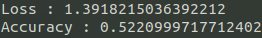
\includegraphics{self_assign_1.png}}
         \caption{自己設定課題 始めの結果}\label{picture:self_assign_1}
        \end{center}
    \end{figure}

    \ref{手書き文字認識}では90\%を超えていたが、\ref{自己設定課題}では難易度が高い画像を選んだことで、52\%と
    かなり正答率が下がった事がわかる。これを改善していく。
    \end{subsection}

    \begin{subsection}{修正点}
    \begin{lstlisting}
#!/usr/bin/python3
# coding: UTF-8
import cv2
import tensorflow.keras
from tensorflow.keras.datasets import cifar10
from tensorflow.keras.models import Sequential
from tensorflow.keras.layers import Dense, Dropout, Flatten
from tensorflow.keras.layers import Conv2D, MaxPooling2D
from tensorflow.keras import backend as K

from tensorflow.keras.callbacks import EarlyStopping
from tensorflow.keras.callbacks import ReduceLROnPlateau

early_stopping = EarlyStopping(
    monitor='val_loss',
    min_delta = 0.0,
    patience = 10,
)

reduce_lr = ReduceLROnPlateau(
    monitor = 'val_loss',
    factor = 0.5,
    patience = 2,
    min_lr = 0.0001,
)
(x_train, y_train), (x_valid, y_valid) = cifar10.load_data()

def main():
    x_train = x_train.astype('float32')
    x_train /= 255
    x_valid = x_valid.astype('float32')
    x_valid /= 255

    #x_train = x_train.reshape(x_train.shape[0], x_train.shape[1], x_train.shape[2], 1)
    x_train = x_train.reshape(x_train.shape[0], x_train.shape[1], x_train.shape[2], 3)
    #x_valid = x_valid.reshape(x_valid.shape[0], x_valid.shape[1], x_valid.shape[2], 1)
    x_valid = x_valid.reshape(x_valid.shape[0], x_valid.shape[1], x_valid.shape[2], 3)

    y_1hot_train = tensorflow.keras.utils.to_categorical(y_train, 10)
    y_1hot_valid = tensorflow.keras.utils.to_categorical(y_valid, 10)

    model = Sequential()
    model.add(Conv2D(32, kernel_size = (3,3),
                        activation = 'relu',
                        input_shape = (x_train.shape[1], x_train.shape[2], x_train.shape[3] )))  
    model.add(Conv2D(16, (3,3), activation = 'relu'))
    model.add(MaxPooling2D(pool_size = (2, 2)))
    model.add(Dropout(0.5))
    model.add(Flatten())
    model.add(Dense(256, activation = 'relu'))
    model.add(Dropout(0.2))
    model.add(Dense(64, activation = 'relu'))
    model.add(Dropout(0.2))
    model.add(Dense(32, activation = 'relu'))
    model.add(Dropout(0.3))

    model.add(Dense(10, activation = 'softmax'))

    model.compile(
        loss=tensorflow.keras.losses.categorical_crossentropy,
        optimizer=tensorflow.keras.optimizers.Adam(),
        metrics=['accuracy'])

    model.fit(x_train, y_1hot_train,
                batch_size=128,  
                epochs=64,
                verbose=1,
                validation_data=(x_valid, y_1hot_valid),
                callbacks = [early_stopping, reduce_lr],)

    score = model.evaluate(x_valid, y_1hot_valid, verbose=0)
    print('Loss :', score[0])
    print('Accuracy :', score[1])

if __name__ == '__main__':
    main()        
    \end{lstlisting}

    まずは
    \begin{lstlisting}
model.add(Conv2D(32, (3, 3), activation = 'relu'))
    \end{lstlisting}
    とあるように、\verb|Conv2D()|の第1引数を8から32に変更した。
    すると次のようになった。

    \begin{figure}[H]
        \begin{center}
         \resizebox{12cm}{!}{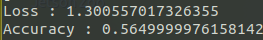
\includegraphics{self_assign_2.png}}  %pngファイルでも表示出来ることが判明した
         \caption{自己設定課題 2回目の結果}\label{picture:self_assign_2}
        \end{center}
    \end{figure}

    多少正答率が上がった。\\
    次に、
    \begin{lstlisting}
model.fit(x_train, y_1hot_train,
    batch_size=128,  
    epochs=16,
    verbose=1,
    validation_data=(x_valid, y_1hot_valid))
    \end{lstlisting}
    とあるように、\verb|epochs|の数を4から16に増やした。すると、次のようになった。
    \begin{figure}[H]
        \begin{center}
         \resizebox{12cm}{!}{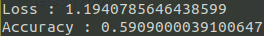
\includegraphics{self_assign_3.png}}
         \caption{自己設定課題 3回目の結果}\label{picture:self_assign_3}
        \end{center}
    \end{figure}

    続いて、
    \begin{lstlisting}
model = Sequential()
model.add(Conv2D(32, kernel_size = (3,3),
                    activation = 'relu',
                    input_shape = (x_train.shape[1], x_train.shape[2], x_train.shape[3] )))  
model.add(Conv2D(16, (3,3), activation = 'relu'))
model.add(MaxPooling2D(pool_size = (2, 2)))
#model.add(Dropout(0.25))
model.add(Flatten())
model.add(Dense(128, activation = 'relu'))
#model.add(Dropout(0.5))
model.add(Dense(64, activation = 'relu'))
#model.add(Dropout(0.5))
model.add(Dense(32, activation = 'relu'))
#model.add(Dropout(0.5))
model.add(Dense(10, activation = 'softmax'))
    \end{lstlisting}
    とあるようにMNIST識別用モデルに層を追加した。
    \verb|Dropout()|は一旦コメントアウトして考える。
    ここでは、追加した項目が多いので、比較用に変更前のプログラムも貼り付ける。

    \begin{lstlisting}
model = Sequential()
    model.add(Conv2D(32, kernel_size = (3,3),
                        activation = 'relu',
                        input_shape = (x_train.shape[1], x_train.shape[2], x_train.shape[3] )))  
    model.add(Conv2D(16, (3, 3), activation = 'relu'))
    model.add(MaxPooling2D(pool_size = (2, 2)))
    model.add(Dropout(0.25))
    model.add(Flatten())
    model.add(Dense(32, activation = 'relu'))
    model.add(Dropout(0.5))
    model.add(Dense(10, activation = 'softmax'))
    \end{lstlisting}

    実行結果を以下に示す。
    \begin{figure}[H]
        \begin{center}
         \resizebox{12cm}{!}{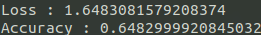
\includegraphics{self_assign_4.png}}
         \caption{自己設定課題 4回目の結果}\label{picture:self_assign_4}
        \end{center}
    \end{figure}

    ここで、正答率は確かに向上しているが、\verb|Loss|が増えてしまった。これについて考える。\\
    グラフを以下に示す。(出典 : \cite[ドロップアウト]{ドロップアウト})\\
    \begin{figure}[H]
        \begin{center}
         \resizebox{12cm}{!}{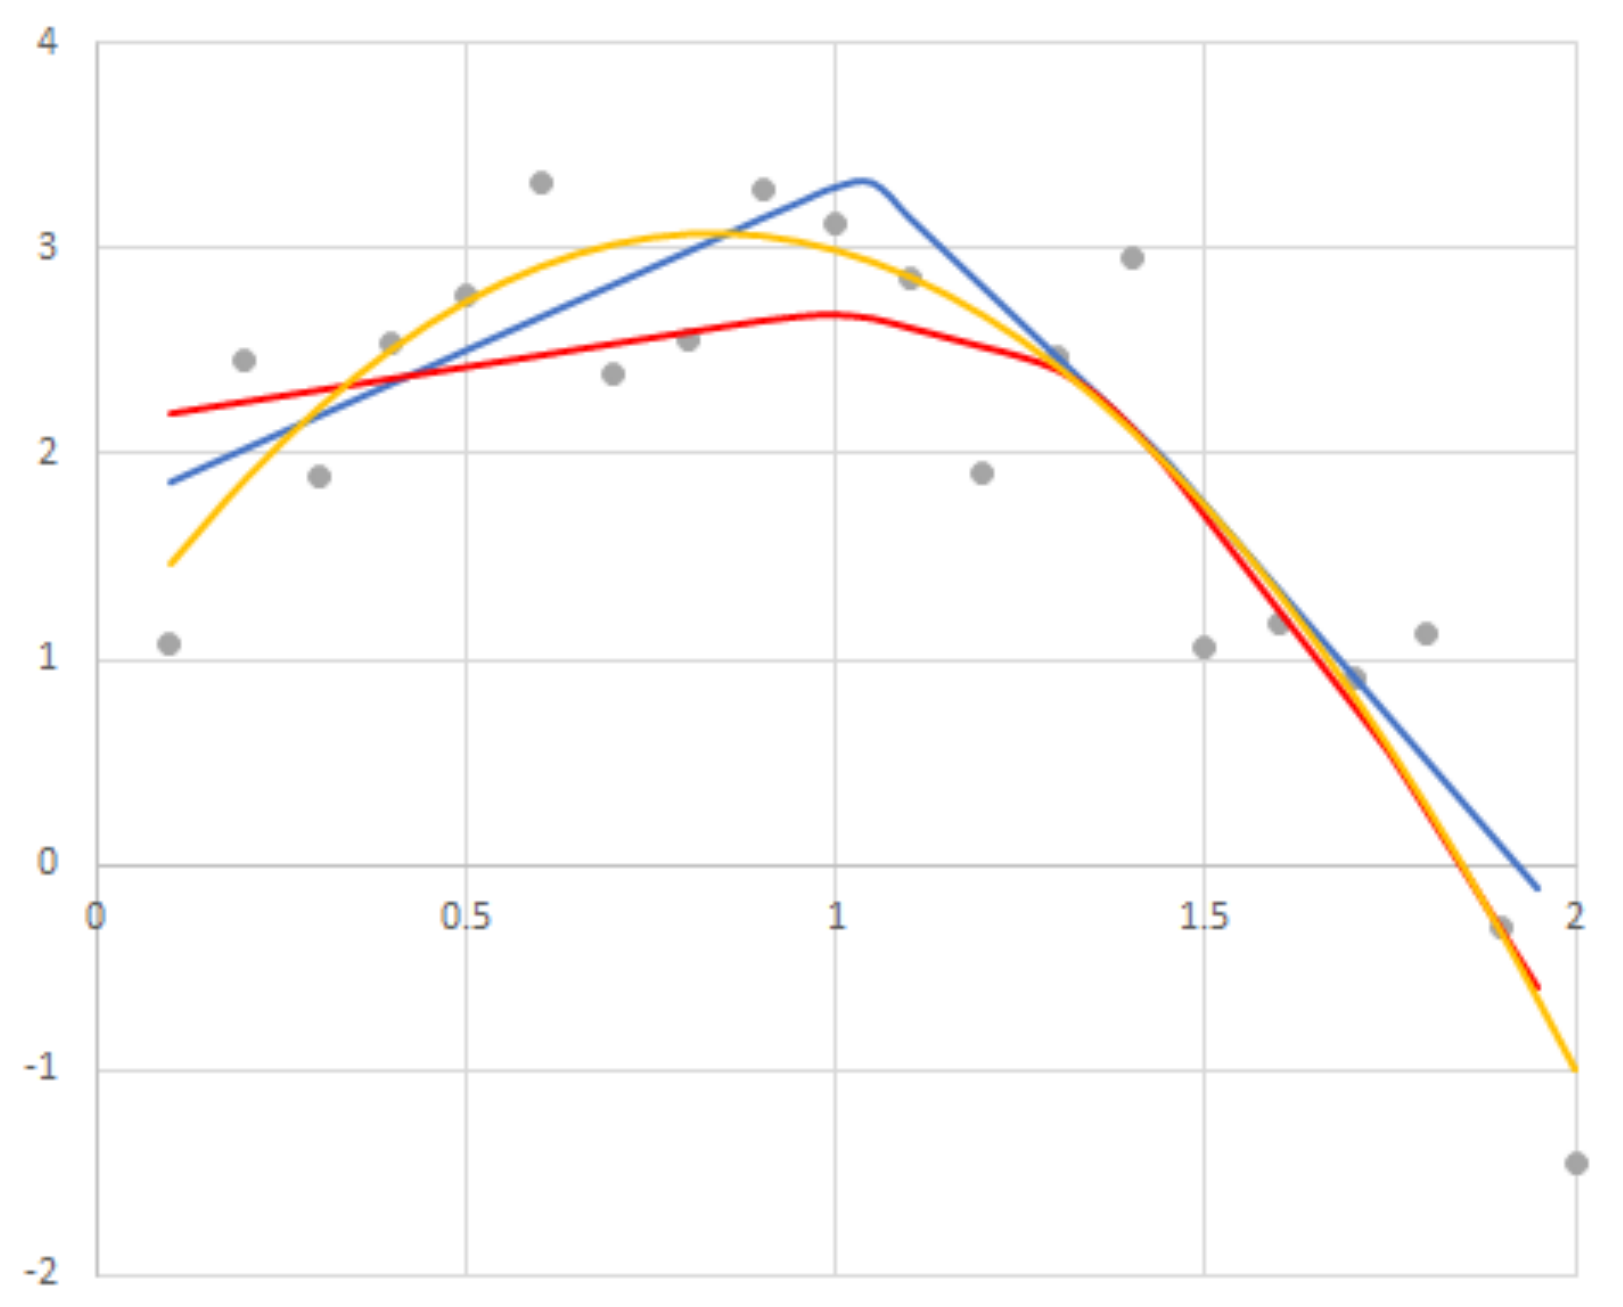
\includegraphics{dropout.png}}
         \caption{ドロップアウトの参考グラフ}\label{picture:dropout}
        \end{center}
    \end{figure}
    ここで、各グラフの説明をすると、
    \begin{itemize}
        \item \textcolor{yellow}{黄色} : 2次関数
        \item \textcolor{red}{赤色} : ドロップアウトあり
        \item \textcolor{blue}{青色} : ドロップアウトなし
    \end{itemize}
    である。
    このグラフから分かる通りドロップアウトが無いと、カクンと折れ曲がった少し急なグラフとなる。
    それにより、極端な学習が行われてしまい、\verb|Loss|(損失値・誤差)は大きくなったと考えられる。\\

    ということで、\verb|Dropout()|に適切な引数を渡して実行してみる。
    \begin{lstlisting}
model.add(Conv2D(32, kernel_size = (3,3),
    activation = 'relu',
    input_shape = (x_train.shape[1], x_train.shape[2], x_train.shape[3] )))  
    model.add(Conv2D(16, (3,3), activation = 'relu'))
    model.add(MaxPooling2D(pool_size = (2, 2)))
    model.add(Dropout(0.3))
    model.add(Flatten())
    model.add(Dense(128, activation = 'relu'))
    model.add(Dropout(0.5))
    model.add(Dense(64, activation = 'relu'))
    model.add(Dropout(0.5))
    model.add(Dense(32, activation = 'relu'))
    model.add(Dropout(0.5))
    model.add(Dense(10, activation = 'softmax'))
    \end{lstlisting}

    結果は次のようになった。
    \begin{figure}[H]
        \begin{center}
         \resizebox{12cm}{!}{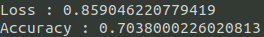
\includegraphics{self_assign_5.png}}
         \caption{自己設定課題 5回目の結果}\label{picture:self_assign_5}
        \end{center}
    \end{figure}
    先程の図\ref{picture:self_assign_4}の結果と比較して、\verb|Loss|の値がおおよそ1.65から0.859になった。
    改善したことが分かる。\\
    また、\verb|Accuracy|も70\%を越えている。

    更に\verb|Accuracy|を向上させるために、\verb|Dropout()|の引数を色々と変更して試してみる。
    しかし、最高で71\%とあまり改善しなかった。
    その時のプログラムを以下に示す。
    \begin{lstlisting}
model.add(Conv2D(32, kernel_size = (3,3),
    activation = 'relu',
    input_shape = (x_train.shape[1], x_train.shape[2], x_train.shape[3] )))  
    model.add(Conv2D(16, (3,3), activation = 'relu'))
    model.add(MaxPooling2D(pool_size = (2, 2)))
    model.add(Dropout(0.5))
    model.add(Flatten())
    model.add(Dense(256, activation = 'relu'))
    model.add(Dropout(0.2))
    model.add(Dense(64, activation = 'relu'))
    model.add(Dropout(0.3))
    model.add(Dense(32, activation = 'relu'))
    model.add(Dropout(0.3))
    model.add(Dense(10, activation = 'softmax'))
    \end{lstlisting}

    後はこの条件下で\verb|epochs|の値を過学習にならない程度に上げて、更なる\verb|Accuracy|の改善を目指す。
    \verb|epochs| = 64で試す。
    結果は次のようになった。
    \begin{figure}[H]
        \begin{center}
         \resizebox{12cm}{!}{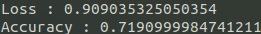
\includegraphics{self_assign_6.png}}
         \caption{自己設定課題 6回目の結果}\label{picture:self_assign_6}
        \end{center}
    \end{figure}

    この数値になった過程について、Excelで\verb|accuracy|のグラフをプロットしたのでその結果も貼る。
    \begin{figure}[H]
        \begin{center}
         \resizebox{12cm}{!}{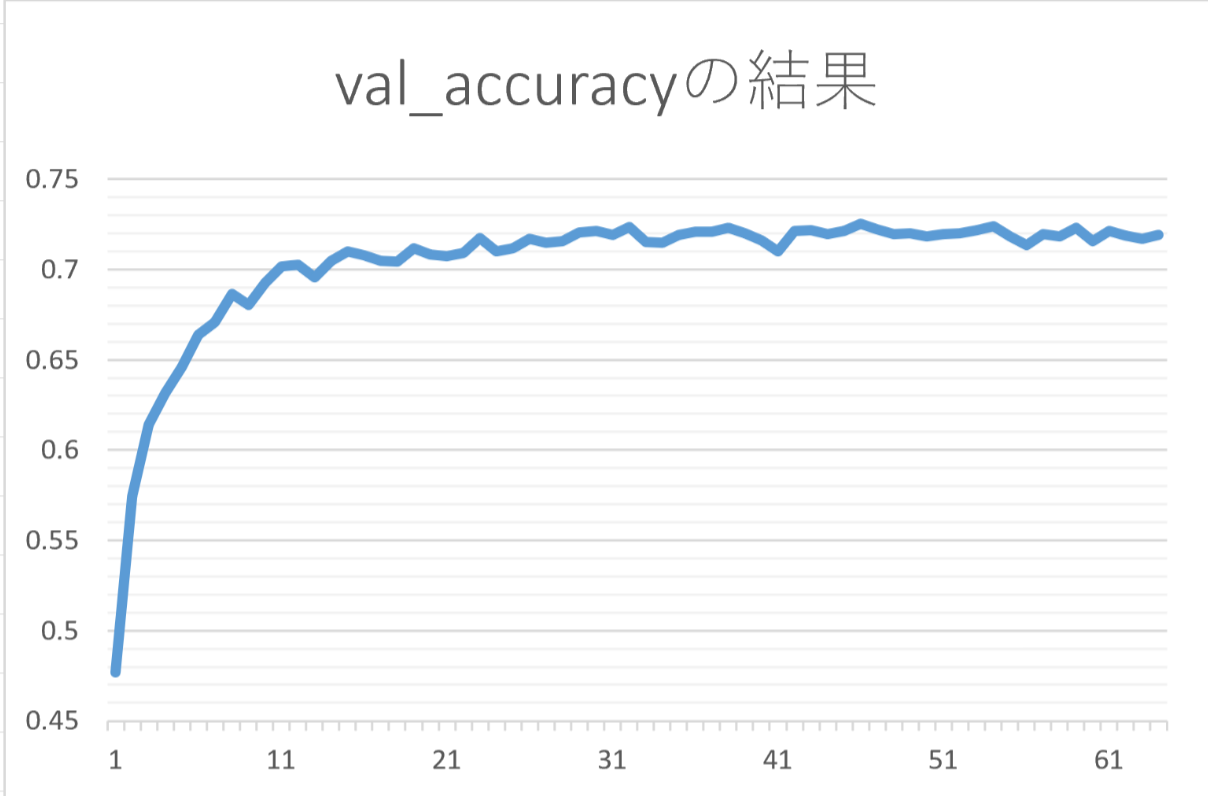
\includegraphics{val_accuracy_graph.png}}
         \caption{val\_accuracyの結果をExcelでプロット}\label{picture:val_accuracy_graph}
        \end{center}
    \end{figure}
    72\%で頭打ちになっている事が分かる。また、\verb|loss|のグラフも書いたので貼る。
    \begin{figure}[H]
        \begin{center}
         \resizebox{12cm}{!}{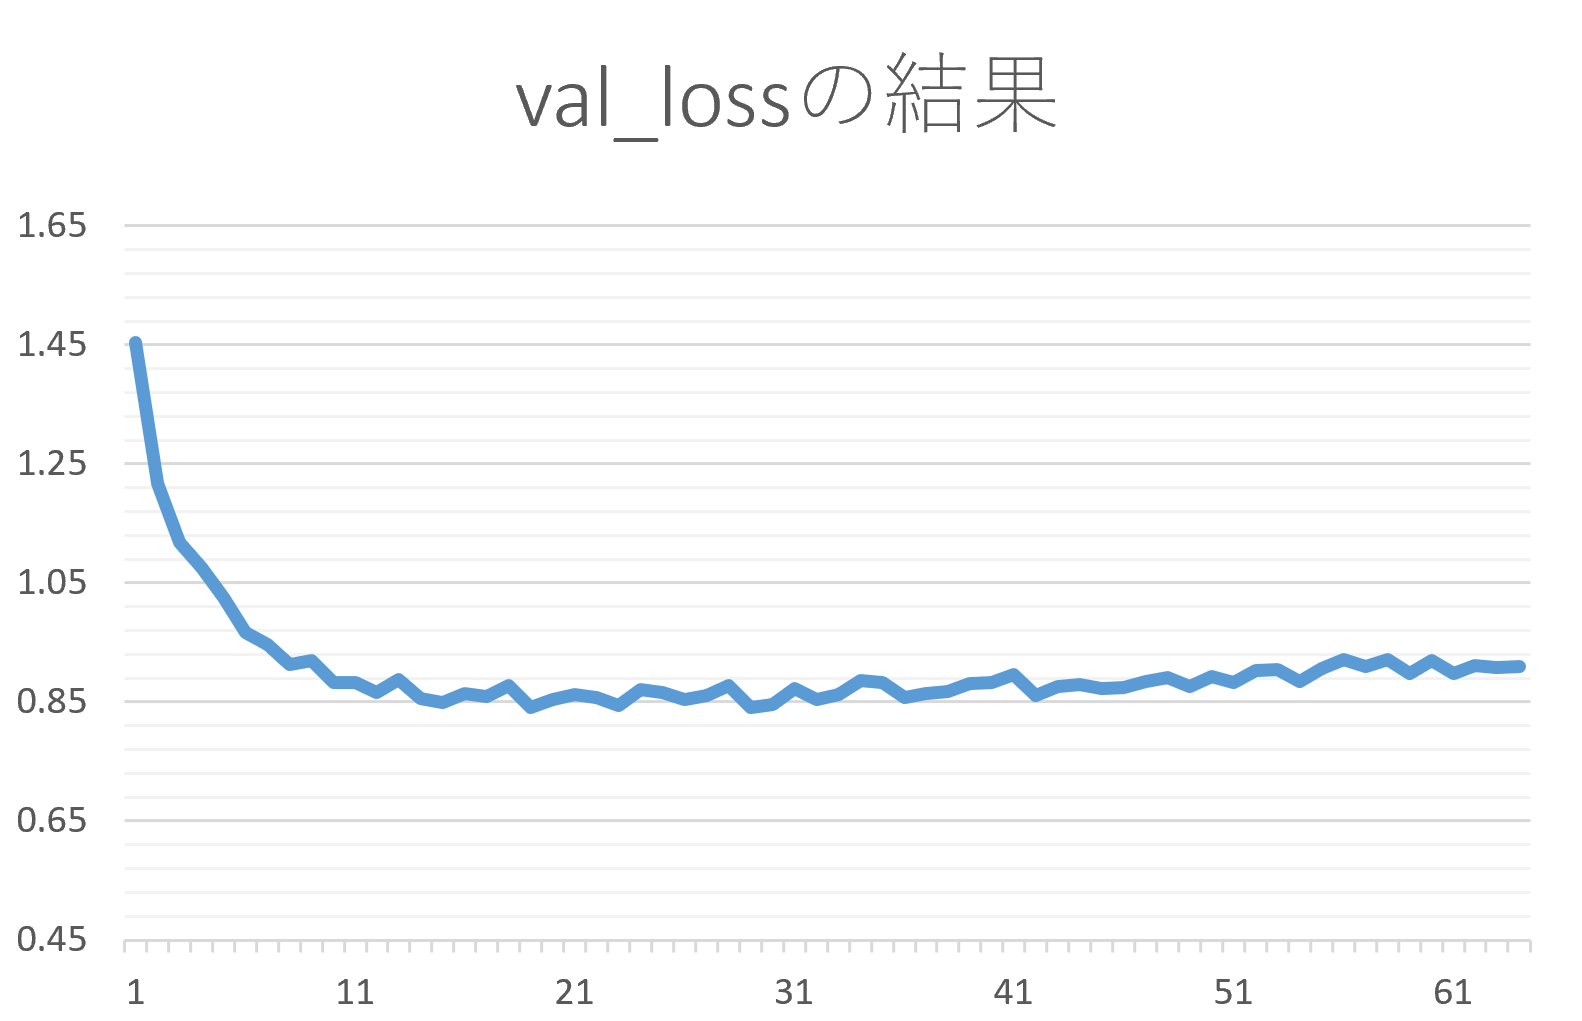
\includegraphics{val_loss_graph.png}}
         \caption{val\_lossの結果をExcelでプロット}\label{picture:val_loss_graph}
        \end{center}
    \end{figure}
    図\ref{picture:val_loss_graph}から分かるように、\verb|val_loss|が全然減っていない。
    むしろ増えているようにも見える。これは、過学習が原因だと考えられる。\\
    つまり、特定のデータにのみ強くなってしまい、その他のデータに対応する力が低下していることである。
    (出典 : \cite[過学習]{過学習})\\

    ここで、過学習対策として、\verb|tensorflow.keras.callbacks|を使用した。
    この関数を使用することで、何エポック改善されなかったら学習率を下げるといったことができ、過学習を抑制できる。\\
    この関数を使用するため、プログラムの\verb|import|部分で
    \begin{lstlisting}
from tensorflow.keras.callbacks import EarlyStopping
from tensorflow.keras.callbacks import ReduceLROnPlateau
    \end{lstlisting}
    と書いた、また関数\verb|early_stopping(), reduce_lr()|も追加した。
    \begin{lstlisting}
early_stopping = EarlyStopping(
        monitor='val_loss',
        min_delta=0.0,
        patience=10,
)

# val_lossの改善が2エポック見られなかったら、学習率を0.5倍する。
reduce_lr = ReduceLROnPlateau(
        monitor='val_loss',
        factor=0.5,
        patience=2,
        min_lr=0.0001
)
    \end{lstlisting}
    更に、
    \begin{lstlisting}
model.fit(x_train, y_1hot_train,
    batch_size=128,  
    epochs=32,
    verbose=1,
    validation_data=(x_valid, y_1hot_valid))
    \end{lstlisting}
    に対して
    \begin{lstlisting}
model.fit(x_train, y_1hot_train,
    batch_size=128,  
    epochs=32,
    verbose=1,
    validation_data=(x_valid, y_1hot_valid),
    callbacks=[early_stopping, reduce_lr],)
    \end{lstlisting}
    のように変更した。つまり、\verb|callbacks|の部分を追加した。
    この関数を定義する上で参考にしたサイトはこちらである。(出典 : \cite[学習率を減らす方法]{学習率を減らす方法})\\

    このプログラムを実行すると、以下のような結果となった。
    \begin{figure}[H]
        \begin{center}
         \resizebox{12cm}{!}{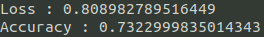
\includegraphics{self_assign_7.png}}
         \caption{自己設定課題 7回目の結果}\label{picture:self_assign_7}
        \end{center}
    \end{figure}

    Excelで過程をプロットした。
    \begin{figure}[H]
        \begin{center}
         \resizebox{12cm}{!}{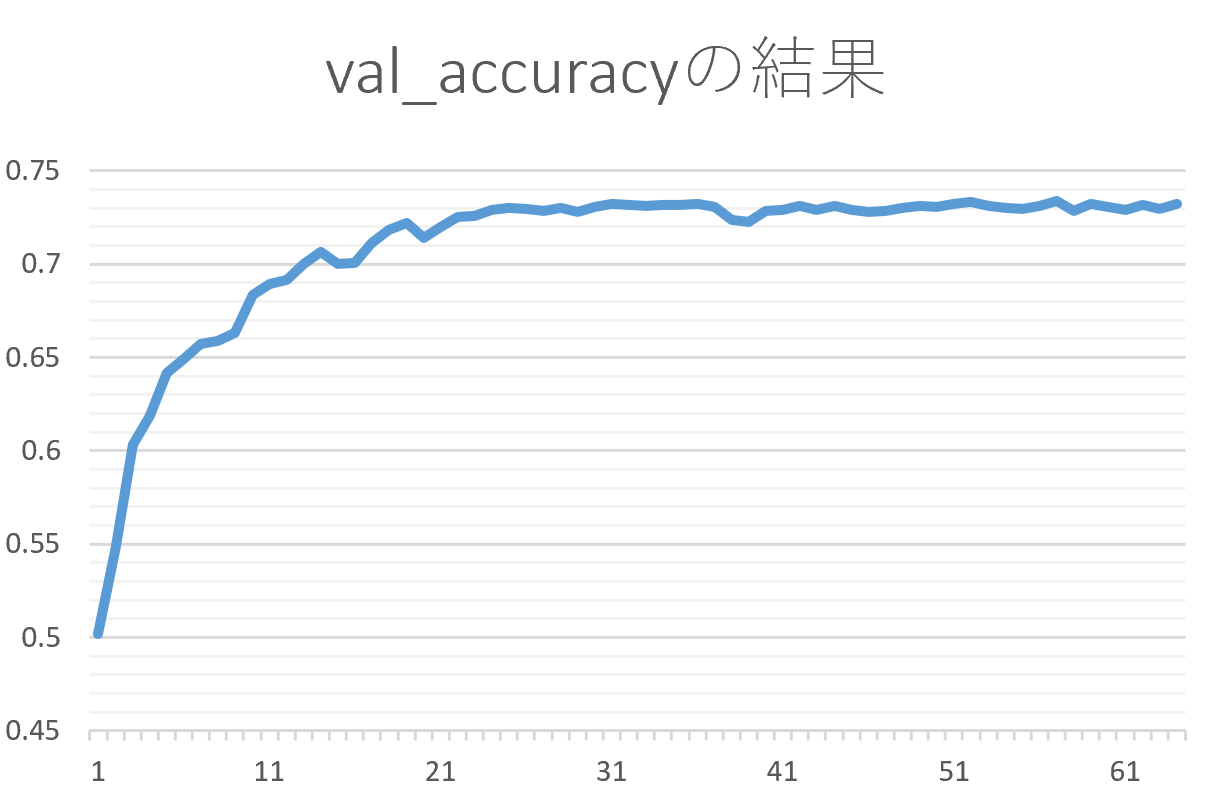
\includegraphics{after_val_accuracy_graph.png}}
         \caption{val\_accuracyの結果をExcelでプロット}\label{picture:after_val_accuracy_graph}
        \end{center}
    \end{figure}
    \begin{figure}[H]
        \begin{center}
         \resizebox{12cm}{!}{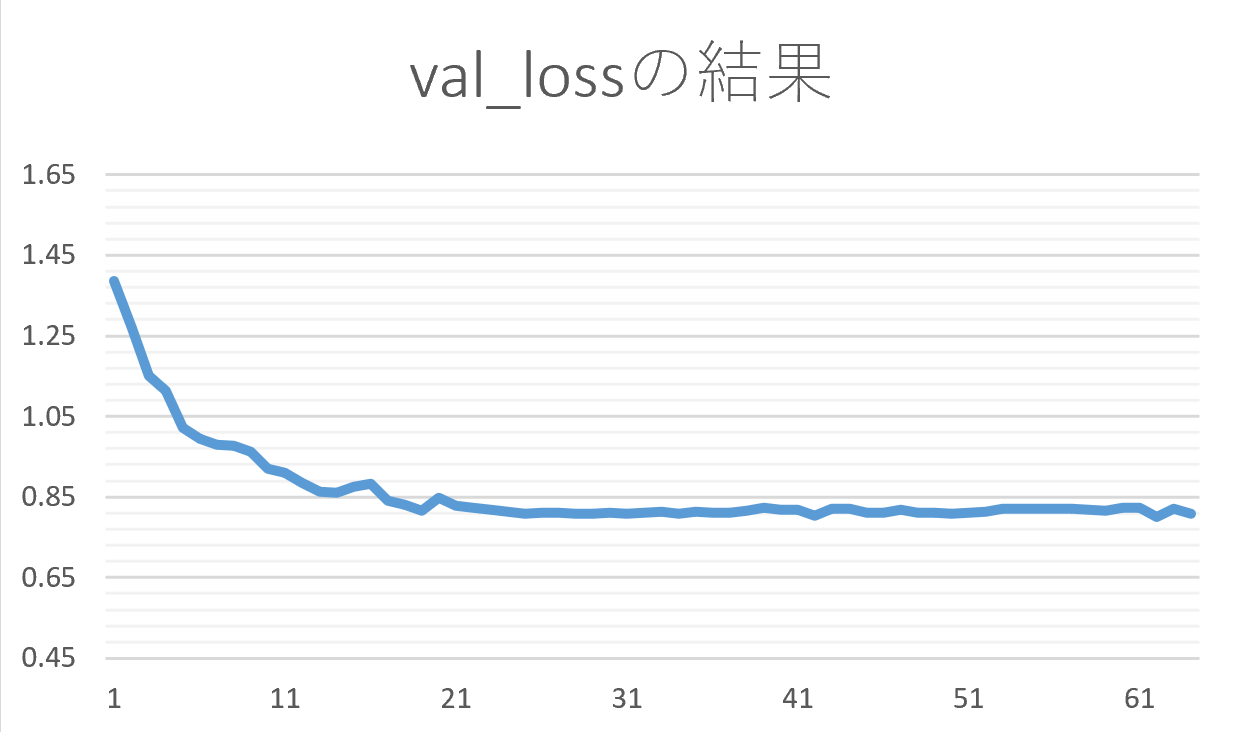
\includegraphics{after_val_loss_graph.png}}
         \caption{val\_lossの結果をExcelでプロット}\label{picture:after_val_loss_graph}
        \end{center}
    \end{figure}
    過学習が抑制されていることが分かる。
    \end{subsection}

    \begin{subsection}{まとめ}
        最後の課題である自己設定課題は、より難しいデータセットへの適用にして、CIFAR-10について行った。
        その際課題3(手書き文字認識)から変更したところは、
        \begin{enumerate}
            \item \verb|epochs|の数を4から16に増やした。
            \item MNIST識別用モデルに層を追加した。
            \item \verb|Dropout|に適切な引数を渡した。
            \item 過学習を防ぐため、\verb|tensorflow.keras.callbacks|を使用した。
        \end{enumerate}
        である。
        最終的な結果は
        \begin{figure}[H]
            \begin{center}
             \resizebox{12cm}{!}{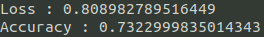
\includegraphics{self_assign_7.png}}
             \caption{自己設定課題 7回目の結果}
            \end{center}
        \end{figure}
        であり、70\%を越える事ができた。また、
        \begin{figure}[H]
            \begin{center}
             \resizebox{12cm}{!}{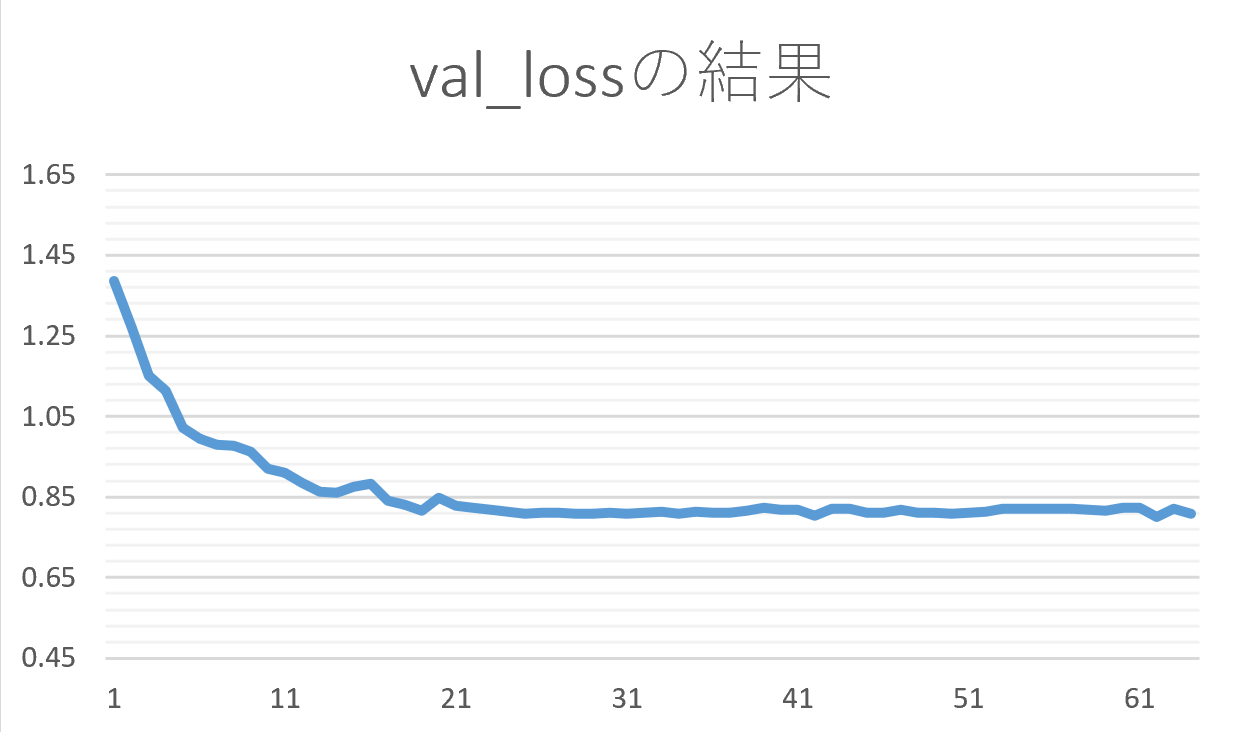
\includegraphics{after_val_loss_graph.png}}
             \caption{val\_lossの結果をExcelでプロット}
            \end{center}
        \end{figure}
        のグラフから分かる通り、過学習を抑制することもできた。\\
        ただ、過学習の抑制はあくまでグラフのブレを抑制するだけであり、80\%を越えるなどといった高い正答率は
        得られなかった。もっと高い正答率を得ようとするのならば、
        \begin{lstlisting}
x = Conv2D(64,(3,3),padding = "SAME",activation= "relu")(inputs)
x = Conv2D(64,(3,3),padding = "SAME",activation= "relu")(x)
x = BatchNormalization()(x)
x = Conv2D(64,(3,3),padding = "SAME",activation= "relu")(x)
x = MaxPooling2D()(x)
x = Dropout(0.25)(x)

x = Conv2D(128,(3,3),padding = "SAME",activation= "relu")(x)
x = Conv2D(128,(3,3),padding = "SAME",activation= "relu")(x)
x = BatchNormalization()(x)
x = Conv2D(128,(3,3),padding = "SAME",activation= "relu")(x)
x = MaxPooling2D()(x)
x = Dropout(0.25)(x)

x = Conv2D(256,(3,3),padding = "SAME",activation= "relu")(x)
x = Conv2D(256,(3,3),padding = "SAME",activation= "relu")(x)
x = BatchNormalization()(x)
x = Conv2D(256,(3,3),padding = "SAME",activation= "relu")(x)
x = Conv2D(256,(3,3),padding = "SAME",activation= "relu")(x)
x = Conv2D(256,(3,3),padding = "SAME",activation= "relu")(x)
x = BatchNormalization()(x)
x = Conv2D(512,(3,3),padding = "SAME",activation= "relu")(x)
x = Conv2D(512,(3,3),padding = "SAME",activation= "relu")(x)
x = GlobalAveragePooling2D()(x)
        \end{lstlisting}
        (出典 : \cite[正答率の向上]{正答率の向上})\\
        のように層をもっと増やす方法などが考えられるが、これはメモリなどの関係上厳しそうである。

        画像をフィルタに通したり、深層学習の「収束」に当たる再急降下法を学んだり、画像を機械に認識させて何の画像かを当てることを
        通して、機械学習の基礎がどのように行われているのかが分かった。
        更に、\ref{自己設定課題}の自己設定課題で\verb|tensorflow.keras.callbacks|を使って過学習を抑制するなど、問題解決の力も付いた。
    \end{subsection}

\end{section}

\begin{thebibliography}{9}   % 参考文献

\bibitem{畳み込み演算}
畳み込み演算\\
\verb|https://axa.biopapyrus.jp/deep-learning/cnn/convolution.html|\\
2023/1/29閲覧\\

\bibitem{再急降下法}
再急降下法\\
\verb|https://kamino.hatenablog.com/entry/steepest_gauss|\\
2023/1/29閲覧\\


\bibitem{Adamを選択した理由}
Adamを選択した理由\\
\verb|https://postd.cc/optimizing-gradient-descent/#whichoptimizertochoose|\\
2023/1/29閲覧\\

\bibitem{ドロップアウト}
ドロップアウト\\
\verb|http://marupeke296.com/IKDADV_DL_No11_dropout.html|\\ 
2023/1/30閲覧\\

\bibitem{過学習}
過学習\\
\verb|https://www.tryeting.jp/column/6037/|\\
2023/1/30閲覧\\

\bibitem{学習率を減らす方法}
学習率を減らす方法\\
\verb|https://analytics-note.xyz/machine-learning/reduce-lr-on-plateau/|\\
2023/1/30閲覧\\

\bibitem{正答率の向上}
正答率の向上\\
\verb|https://qiita.com/yy1003/items/c590d1a26918e4abe512|\\
2023/1/30閲覧\\

\end{thebibliography}

\end{document}